\newpage
\section{柔軟外皮を備えたワイヤ駆動式魚ロボットの開発}
前章で述べたように,先行研究\cite{kyu}では屈曲可能な胴体を持ち,柔軟外皮を装着して完全防水を可能にした魚ロボットの開発に成功した.しかし,リンクと外皮に隙間ができてしまい,
リンクの動きを外皮にうまく伝えることができなかった.そこで本研究では魚らしいしなやかな動きを可能にするワイヤ駆動式の魚ロボットをベースにリンクに外皮を追従させ,尾びれのみならず
胴体部まで振って泳ぐことが可能なロボットの開発を目指す.本章ではその予備的な開発として,昨年度卒業研究を参考に外皮を持たないワイヤ駆動式魚型ロボットを開発し,柔軟外皮をどのよう
に組み合わせるべきかなどについて検討を行う.
\subsection{ワイヤ駆動式魚型ロボットの動作原理}
昨年度卒業研究で提案され,本研究でも採用したワイヤ駆動の動作原理を記す.ロボット前方にはプーリを取り付けたサーボモータを配置し,胴体部には弾性体とそれに固定した骨格リンクを配置する.
ワイヤはプーリーから骨格リンクに設けられた穴を通って尾びれ付け根まで伸びており,プーリーを回してワイヤを巻き取ることによって弾性体が曲がり,胴体部を屈曲させることができる.それを左
右に繰り返すことで遊泳を可能にする(図\ref{fig:waiyakudou})

\begin{figure}[b]
   \centering
   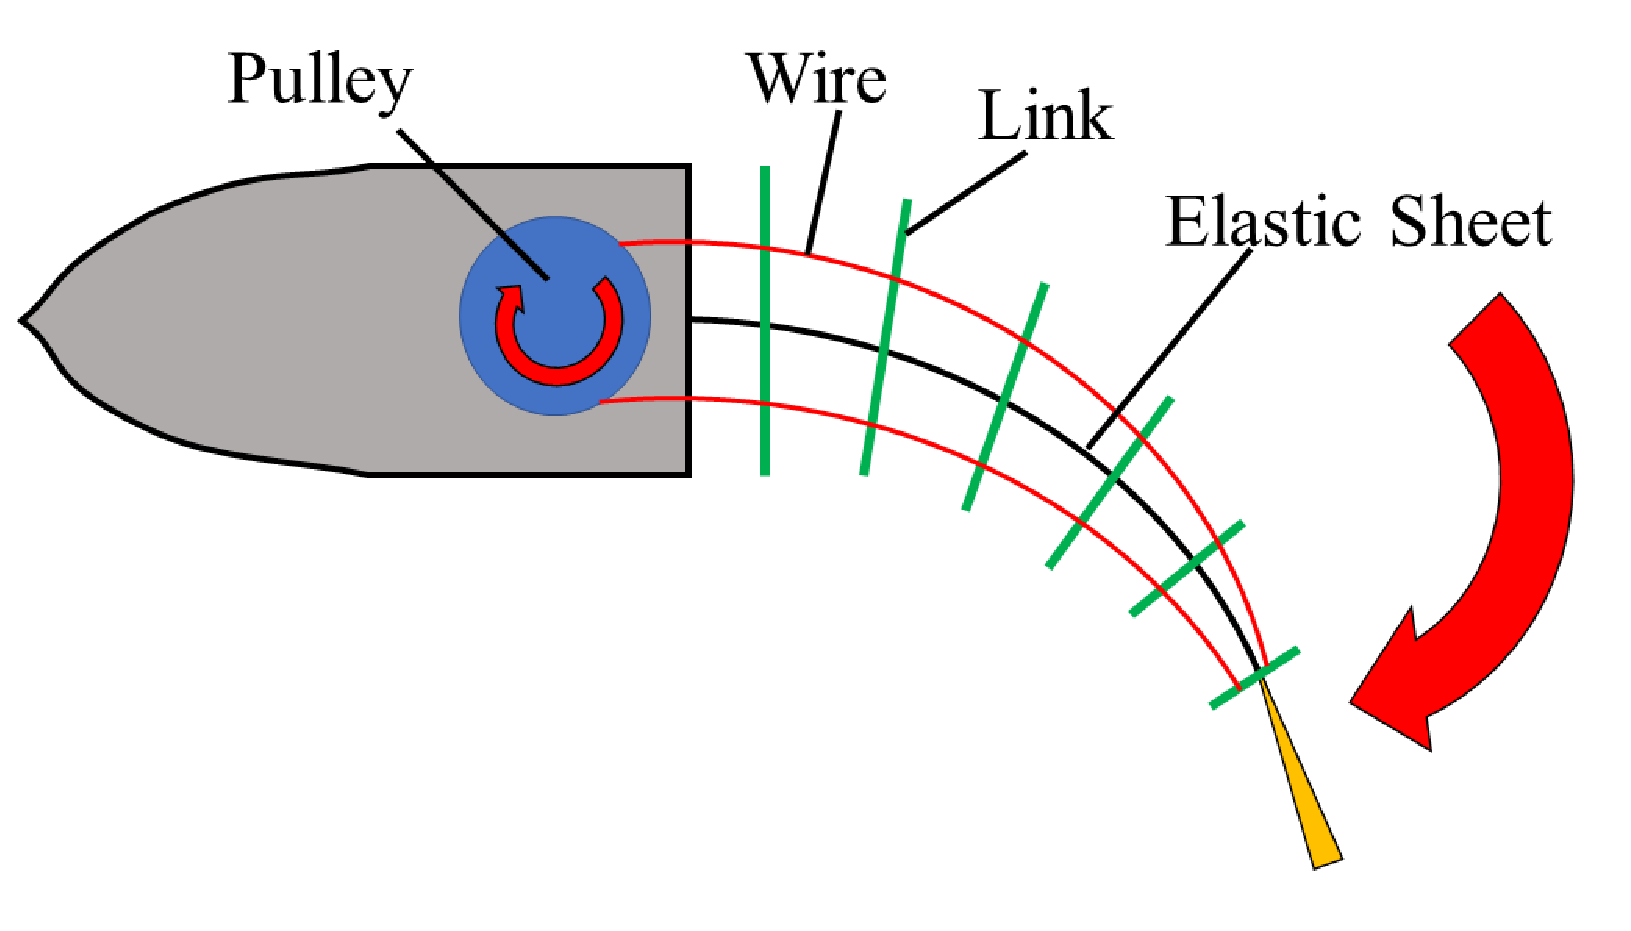
\includegraphics[width=0.6\linewidth]{chapters/picture/waiyakudou.eps}
   \caption{ワイヤ駆動のイメージ}
   \label{fig:waiyakudou}
\end{figure}

\subsection{試作機}
\subsubsection{試作機の作製}
まず,昨年度卒業研究を参考にして試作機を作製した.図\ref{fig:sisaku}に外観を,図\ref{fig:kouzou_sisaku}に構造を示す.全長は530 mm,重量は478 gである.試作機は頭部と胴体部の二つ
の部分で構成している.

頭部には制御回路とバッテリーを搭載しており,えらにあたる部分には防水仕様(IP67)の サーボモータ(Flash Hobby, M45CHW)を配置している.サーボモータは270°回転できるようになっている.
使用マイコンはM5Stamp Pico(M5Stack Technology 社),使用バッテリーはマイコン用の3.7 V,サーボモータ用の7.4 Vの二つのLi-ionバッテリーを使用している.そのため,頭部は防水が必要となり,
頭部の断面にOリングをはめ込むことによって防水を行っている.頭部はネジ穴が空いたものと,ナット用の穴が空いたものに分かれており,これらはM1.7ネジで固定される.
胴体部は骨格リンク(PLA樹脂)と弾性体(ポリプロピレン板,厚さ0.75 mm),尾びれ(TPU樹脂,厚さ2 mm)で構成されており,骨格リンクは図のように楕円形にして作製し,ワイヤ(ポリエステル製,0.40 mm)
を通す穴を空けている.

\begin{figure}[t]
    \centering
    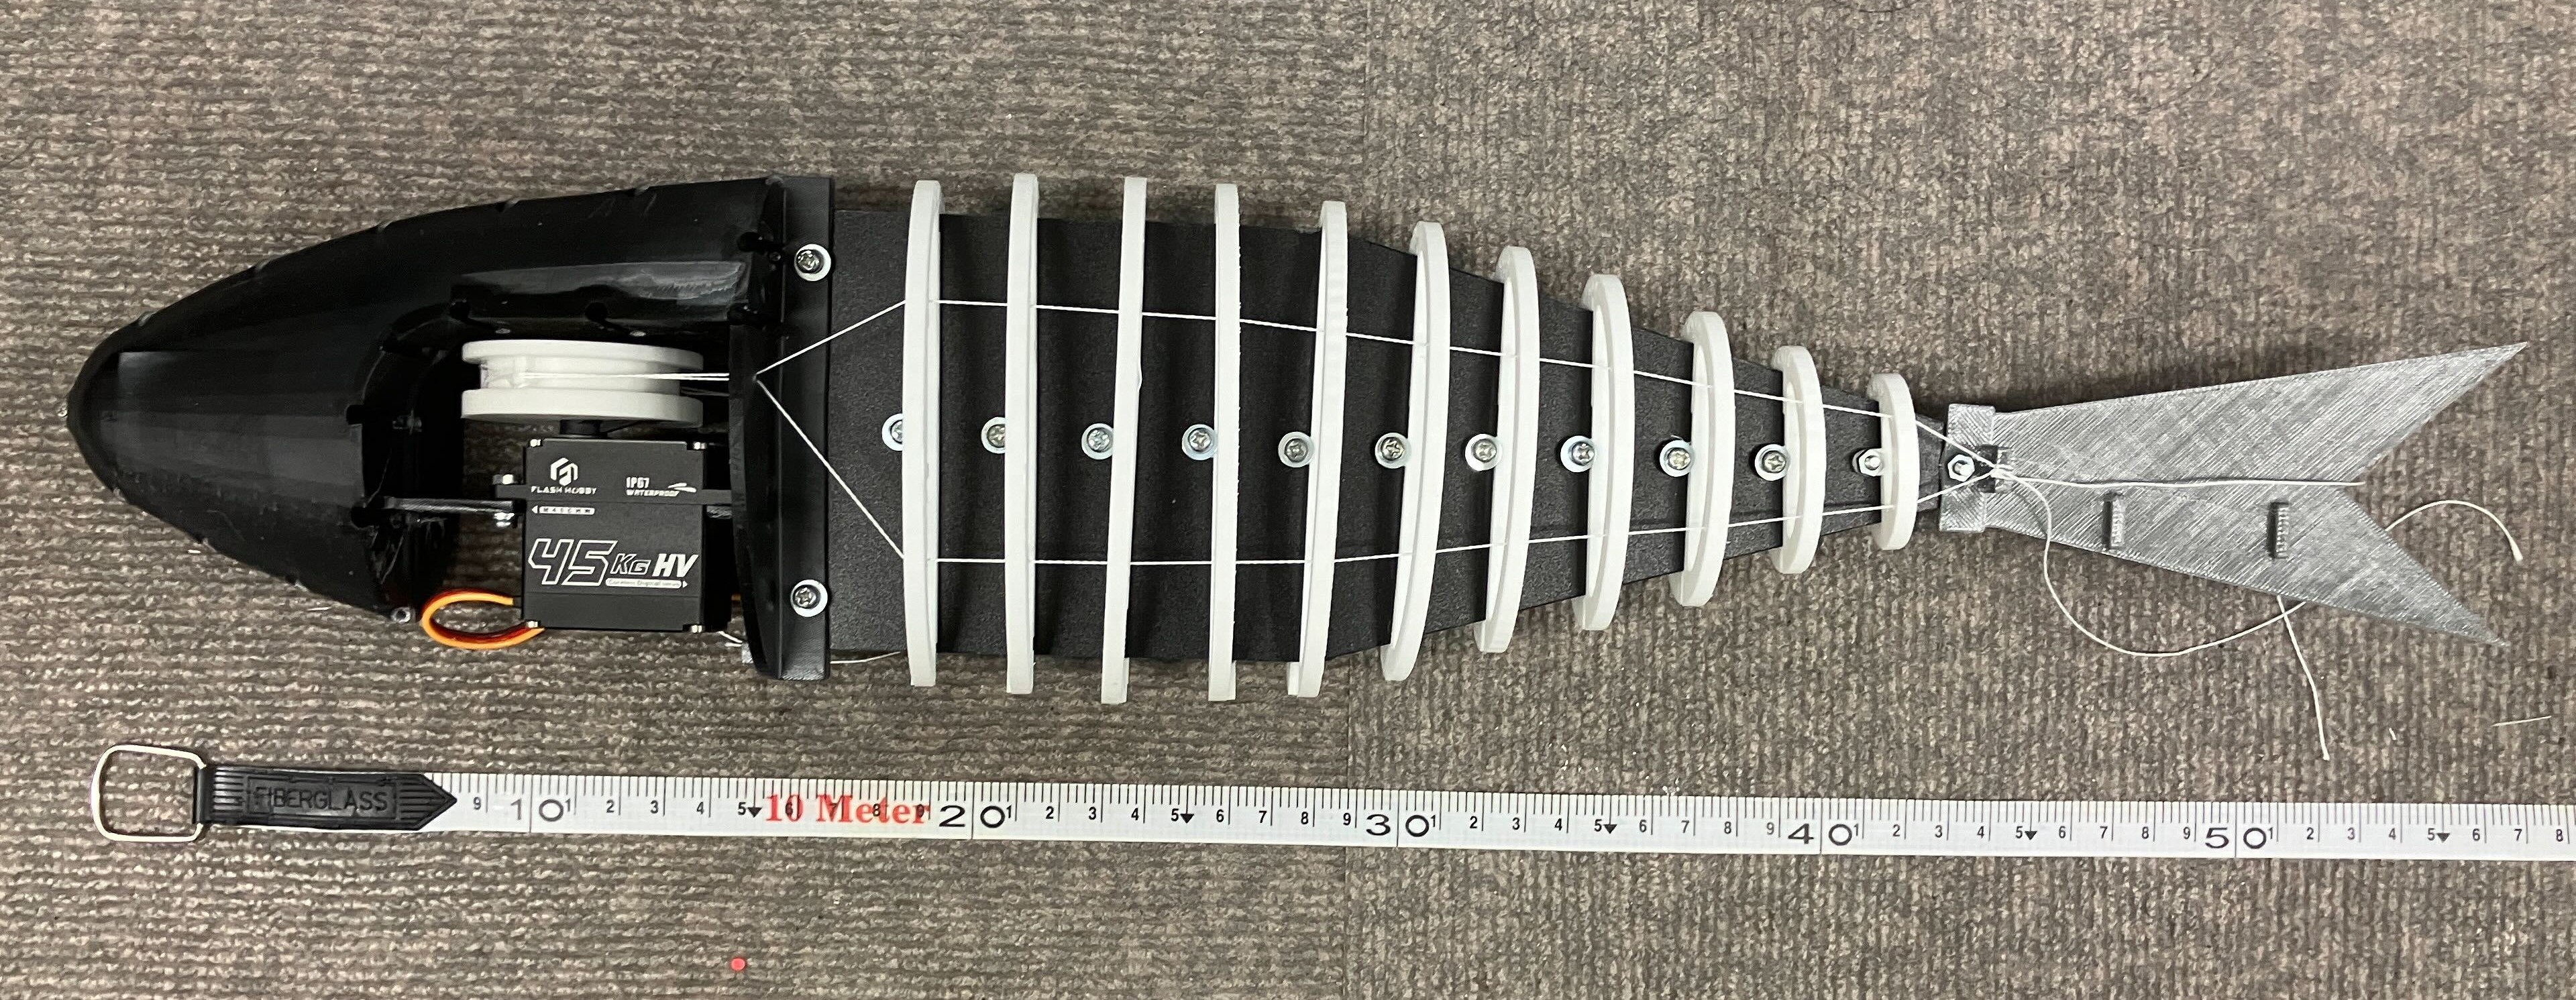
\includegraphics[width=0.80\linewidth]{chapters/picture/sisaku.jpg}
    \caption{試作機の外観}
    \label{fig:sisaku}
\end{figure}
\begin{figure}[t]
    \centering
    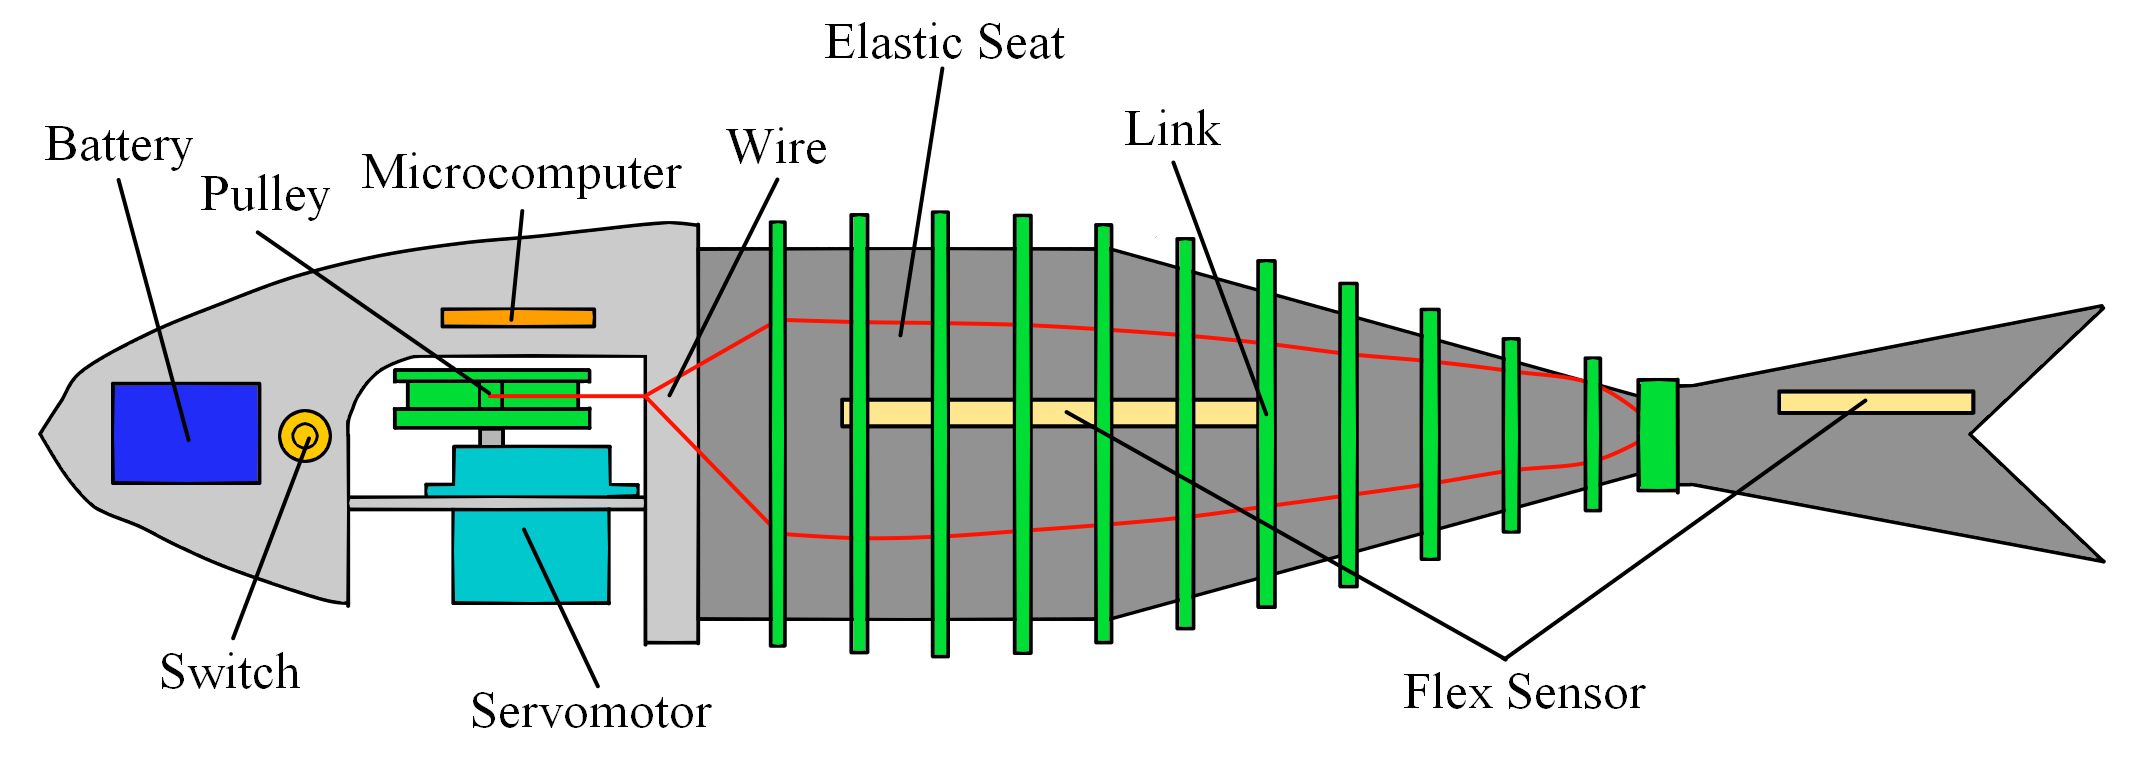
\includegraphics[width=0.80\linewidth]{chapters/picture/tentativeschematic.png}
    \caption{試作機の構造}
    \label{fig:kouzou_sisaku}
\end{figure}
\begin{figure}[t]
    \centering
     \begin{minipage}[b]{0.50\linewidth}
        \centering
        \setPicture{ring.jpg}
        \caption{頭部断面のようす}
        \label{fig:danmen}
     \end{minipage}
     \hspace{0.05\linewidth}
     \begin{minipage}[b]{0.25\linewidth}
        \centering
        \setPicture{jikkilink.png}
        \caption{骨格リンク}
        \label{fig:link_sen}
     \end{minipage}
\end{figure}

\subsubsection{防水テスト・遊泳テスト}
機体完成後,防水テストと遊泳テストを行った.まず防水テストは水没すると赤くなるシールを頭部内部に貼り,水深120 mmの水槽で2 分間沈める防水テストを7回行った.それぞれねじの締め具合や
頭部の歪みを直しながらテストをしたが,完全な防水はできず,7回目で頭部下方のみの浸水にとどまったのでこれで防水できていると判断した(図\ref{fig:bousuitest_sisaku}).
次に遊泳テストを行った.遊泳テストの様子を図\ref{fig:test_sisaku}に示す.

\begin{figure}[t]
    \centering
    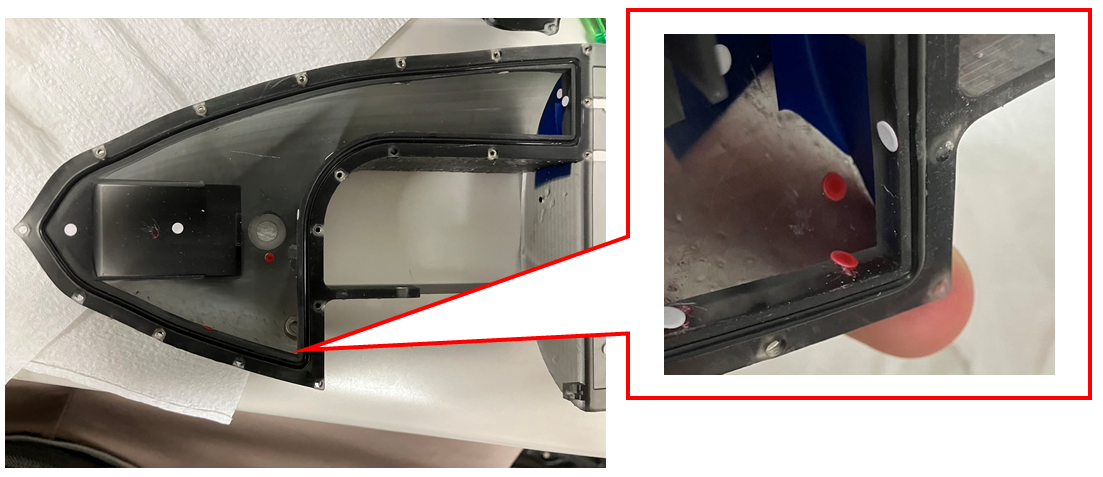
\includegraphics[width=0.80\linewidth]{chapters/picture/bousuitest.png}
    \caption{頭部下方浸水のようす}
    \label{fig:bousuitest_sisaku}
\end{figure}
\begin{figure}[t]
    \centering
    \setPicture{sisakuoyogu2.png}
    \caption{遊泳テストの様子}
    \label{fig:test_sisaku}
\end{figure}

\subsubsection{試作機から得られた知見}
試作機の作製・動作確認を通して得られた知見として,まず,頭部をネジとOリングを用いて防水する方法は完全な防水に至らないと考えられる.また,頭部を固定するネジが多いと,バッテリー交換が
しにくく,メンテナンス性が悪くなるということも分かった.以上のことから防水方法を変更し,メンテナンス性を向上させた頭部に改良することが必要だとわかった.そこで防水を比較的容易にでき,
完全防水可能な柔軟外皮を用いて頭部の防水を行うようにする.また,骨格リンクが胴体の形状をなしていることを生かし,骨格リンクをはめられるような溝を胴体外皮内部に作製することでリンクと
外皮の追従を行う.